\documentclass[12pt,aspectratio=169]{beamer}

% ====================================================
% ====================================================
% USEPACKAGES AND IMPORTS
% ====================================================
% ====================================================

\usepackage[T1]{fontenc}
\usepackage[utf8]{inputenc}
\usepackage[english]{babel}

% tables
\usepackage{tabularx}
\usepackage{colortbl}
\usepackage{multirow}
\usepackage{makecell}

% tikz and colors
\usepackage{tikz}
\usepackage{xcolor}
\usepackage{pgfplots}
\usepackage{pgfplotstable}
\usepackage{tikzsymbols}

\usetikzlibrary{calc}
\usetikzlibrary{trees}
\usetikzlibrary{patterns}
\usetikzlibrary{shadings}
\usetikzlibrary{positioning}
\usetikzlibrary{intersections}
\usepgfplotslibrary{patchplots}
\usepgfplotslibrary{fillbetween}
\usetikzlibrary{decorations.pathreplacing}

\usetikzlibrary{arrows}
\usetikzlibrary{arrows.meta}

\usetikzlibrary{shapes}
\usetikzlibrary{shapes.arrows}
\usetikzlibrary{shapes.callouts}
\usetikzlibrary{shapes.symbols}
\usetikzlibrary{shapes.geometric}

% boxes
\usepackage[many]{tcolorbox}

% math packages and fonts
\usepackage{bm}
\usepackage{ccfonts}
\usepackage{eulervm}
\usepackage{amsmath}
\usepackage{amsfonts}
\usepackage{amssymb}
\usepackage{amsthm}
\usepackage{mathtools}
\usepackage{nicefrac}
\usepackage{slashed}
\usepackage{bbold}
\usepackage{array}
\usepackage{cancel}

% algorithms and listings
\usepackage[ruled,vlined,linesnumbered]{algorithm2e}
\usepackage{listings}
\usepackage{setspace}

\tcbuselibrary{listings}
\tcbuselibrary{breakable}
\tcbuselibrary{skins}

% misc
\usepackage{soul}
\usepackage{pifont}
\usepackage{skull}
\usepackage{multicol}
\usepackage{animate}
\usepackage{hyperref}
\usepackage{wasysym}
\usepackage[absolute,overlay]{textpos}
\usepackage[hang,flushmargin]{footmisc}

% ====================================================
% ====================================================
% LAYOUT AND THEME
% ====================================================
% ====================================================

\usetheme{Copenhagen}

% color definitions
\definecolor{myblue1}{RGB}{35,119,189}
\definecolor{myblue2}{RGB}{95,179,238}
\definecolor{myblue3}{RGB}{129,168,207}
\definecolor{myblue4}{RGB}{26,89,142}

\definecolor{myred1}{RGB}{247,12,12}

% set theme colors
\setbeamercolor*{structure}{fg=myblue1,bg=blue}
\setbeamercolor*{palette primary}{use=structure,fg=white,bg=structure.fg}
\setbeamercolor*{palette secondary}{use=structure,fg=white,bg=structure.fg!75!black}
\setbeamercolor*{palette tertiary}{use=structure,fg=white,bg=structure.fg!50!black}
\setbeamercolor*{palette quaternary}{fg=black,bg=white}

\setbeamertemplate{itemize item}[circle]
\setbeamertemplate{itemize subitem}[circle]
\setbeamertemplate{itemize subsubitem}[circle]

\setbeamertemplate{enumerate item}[circle]
\setbeamertemplate{enumerate subitem}[circle]
\setbeamertemplate{enumerate subsubitem}[circle]

\setbeamercolor{itemize item}{fg=myblue1}
\setbeamercolor{itemize subitem}{fg=myblue1}
\setbeamercolor{itemize subsubitem}{fg=myblue1}

\setbeamertemplate{section in toc}[circle]
\setbeamertemplate{subsection in toc}[circle]
\setbeamerfont{subsection in toc}{size=\scriptsize}

\setbeamercolor{frametitle continuation}{fg=black}

% title graphic -- sap logo and dhbw logo
\titlegraphic{
\includegraphics[scale=0.1]{../03_img/logo_sap}\hspace*{4.75cm}~%
   	
\includegraphics[scale=0.05]{../03_img/logo_dhbw}
}

\makeatletter
% frame title
\defbeamertemplate*{frametitle}{mydefault}[1][left]
{
  	\ifbeamercolorempty[bg]{frametitle}{}{\nointerlineskip}%
  	\nointerlineskip%
 	\@tempdima=\textwidth%
  	\advance\@tempdima by\beamer@leftmargin%
  	\advance\@tempdima by\beamer@rightmargin%
  	\begin{tcolorbox}[
  		enhanced,
  		outer arc=0pt,
  		arc=0pt,
  		boxrule=0pt,
  		top=0pt,
  		bottom=0pt,
  		enlarge left by=-\beamer@leftmargin,
  		enlarge right by=-\beamer@rightmargin,
  		width=\paperwidth,
  		nobeforeafter,
  		interior style={
    			left color=myblue2,
    			right color=white
    		},
  		shadow={0mm}{-0.4mm}{0mm}{black!60,opacity=0.6},    
  		shadow={0mm}{-0.8mm}{0mm}{black!40,opacity=0.4},    
  	]
    	\usebeamerfont{frametitle}%
    	\vbox{}\vskip-1ex%
    	\if@tempswa\else\csname beamer@fte#1\endcsname\fi%
    	\insertframetitle\par%
    	{%
      		\ifx\insertframesubtitle\@empty%
      		\else%
      		{\usebeamerfont{framesubtitle}\usebeamercolor[fg]{black}\insertframesubtitle\strut\par}%
      		\fi
    	}%
    	\vskip-1ex%
    	\if@tempswa\else\vskip-.3cm\fi
  	\end{tcolorbox}%
}

% footline of a frame
\defbeamertemplate*{footline}{mysplit theme}
{%
  	\leavevmode%
  	\hbox{
		\begin{beamercolorbox}[
			wd=.5\paperwidth,ht=2.5ex,dp=1.125ex,leftskip=.3cm plus1fill,rightskip=.3cm
		]{author in head/foot}%
    			\usebeamerfont{author in head/foot}\insertshortauthor\ (\insertinstitute), \insertdate
  		\end{beamercolorbox}%
  		\begin{beamercolorbox}[
			wd=.5\paperwidth,ht=2.5ex,dp=1.125ex,leftskip=.3cm,rightskip=.3cm plus1fil
		]{title in head/foot}%
    			\usebeamerfont{title in head/foot}\insertshorttitle\hfill
    			\insertprefix-\insertframenumber/\inserttotalframenumber\hspace*{0.5em}
  		\end{beamercolorbox}}%
  	\vskip0pt%
}
\makeatother

% ====================================================
% ====================================================
% COMMANDS AND GENERAL DEFINITIONS
% ====================================================
% ====================================================

% page number prefix
\newcommand\insertprefix{}  % empty by default
\newcommand\prefix[1]{\renewcommand\insertprefix{#1}}

% math definitions
% ====================================================
\DeclareMathOperator*{\argmax}{arg\,max}
\DeclareMathOperator*{\argmin}{arg\,min}
\newcommand*\diff{\mathop{}\!\mathrm{d}}

\newcommand*{\vertbar}{\rule[-1ex]{0.5pt}{2.5ex}}
\newcommand*{\horzbar}{\rule[.5ex]{2.5ex}{0.5pt}}

% commands
% ====================================================

% highlight commands
% --------------------------------------------------------------------------------------------------------
% highlight command
\newcommand{\highlight}[1]{\textcolor{myblue1}{\textbf{#1}}}
\newcommand{\highlighttt}[1]{\textcolor{myblue1}{\texttt{#1}}}
\newcommand{\Highlight}[1]{\textcolor{myred1}{\textbf{#1}}}

% blue color boxes (with frame/without frame/without fill)
\newtcolorbox{boxBlue}{colback=myblue1!10!white,colframe=myblue4}
\newtcolorbox{boxBlueNoFrame}{colback=myblue1!10!white,colframe=myblue1!10!white}
\newtcolorbox{boxBlueNoFill}{colback=white,colframe=myblue4}

% font commands
% --------------------------------------------------------------------------------------------------------
\newcommand{\linkstyle}[1]{\underline{\smash{\texttt{#1}}}} 		% style of hyperlinks

% tikz commands
% --------------------------------------------------------------------------------------------------------

% yellow sticky note
\newcommand{\bubble}[3]{
\begin{textblock}{100}(#1, #2)
      	\begin{tikzpicture}
		\node[rectangle,draw=yellow,very thick,fill=yellow!60,align=center] at (0,0) {#3};
	\end{tikzpicture}
\end{textblock}
}

\newcommand{\floattext}[3]{
\begin{textblock}{100}(#1, #2)
      	#3
\end{textblock}
}

\newcommand{\doublecircle}[2]{
	\draw[fill=white,draw=myblue1] (#1,#2) circle (2mm);
	\draw[fill=myblue1,draw=myblue1] (#1,#2) circle (1.5mm);
}

% slide modifiers
% --------------------------------------------------------------------------------------------------------
% mark slide as optional
\newcommand{\optional}{
	\begin{textblock}{100}(0.15,0.30)
      		
\includegraphics[scale=0.2]{../03_img/scream}
    	\end{textblock}
}

% mark slide as important
\newcommand{\important}{
	\begin{textblock}{100}(0.10,0.15)
      		
\includegraphics[scale=0.1]{../03_img/important}
    	\end{textblock}
}

% citation
% --------------------------------------------------------------------------------------------------------
% first argument in {book, online, article}
\newcommand{\literature}[5]{
	\setbeamertemplate{bibliography item}[#1]
	\bibitem{#2}
	\highlight{#3} \\
	\textcolor{darkgray}{\textit{#4}} \\
	\textcolor{black}{#5}
}
% cite content
\newcommand{\citeAuthor}[3]{\vfill\scriptsize\textcolor{lightgray}{#1 \cite{#2} #3}}

% slide architecture
% --------------------------------------------------------------------------------------------------------
% divide frame into two parts
\newcommand{\divideTwo}[4]{
	\begin{minipage}{#1\textwidth}
		#2
	\end{minipage}
	\hfill
	\begin{minipage}{#3\textwidth}
		#4
	\end{minipage}
}

% divide frame into two parts (start on top)
\newcommand{\divideTwoTop}[4]{
	\begin{minipage}[t]{#1\textwidth}
		#2
	\end{minipage}
	\hfill
	\begin{minipage}[t]{#3\textwidth}
		#4
	\end{minipage}
}

% special pages
% --------------------------------------------------------------------------------------------------------
% title page
\newcommand{\maketitlepage}{
	{
		\beamertemplatenavigationsymbolsempty
		\usebackgroundtemplate{%
			\tikz[overlay,remember picture] \node[opacity=0.2, at=(current page.center)] {
  				
\includegraphics[height=\paperheight,width=\paperwidth]{../03_img/processor.jpg}
			};
		}
		\begin{frame}[plain]
			\vspace*{0.75cm}
			\maketitle
			\vfill
			\begin{center}
				\footnotesize Find all slides on \href{https://github.com/DaWe1992/Applied_ML_Fundamentals}{\linkstyle{GitHub}}
			\end{center}
		\end{frame}
	}
}

% divider page
\newcommand{\makedivider}[1]{
	{
		\beamertemplatenavigationsymbolsempty
		\usebackgroundtemplate{%
			\tikz[overlay,remember picture] \node[opacity=0.2, at=(current page.center)] {
  				
\includegraphics[height=\paperheight,width=\paperwidth]{../03_img/processor.jpg}
			};
		}
		\begin{frame}[plain]
			\vfill
			\begin{boxBlue}
				\centering
				\textbf{Section:} \\
				\large \highlight{#1}
			\end{boxBlue}
			\vfill
			\centering
			
\includegraphics[scale=0.05]{../03_img/logo_dhbw.png}
			\vfill
		\end{frame}
	}
}

% overview page
\newcommand{\makeoverview}[1]{
	\begin{frame}{Lecture Overview}{}
		\begin{tabbing}
			\hspace*{3.5cm}\= \kill
			\ifnum #1=1 \highlight{\textbf{Unit I:}} \else \textbf{Unit I:} \fi
			\> \ifnum #1=1 \highlight{Machine Learning Introduction} \else Machine Learning Introduction \fi \\
		\end{tabbing}
	\end{frame}
}

% thank you page
\newcommand{\makethanks}{
	{\beamertemplatenavigationsymbolsempty
	\begin{frame}[plain]
		\vfill
		\begin{boxBlue}
			\centering
			\Large \highlight{Thank you very much for the attention!}
		\end{boxBlue}
		
		\vfill\footnotesize
		\begin{tabbing}
			\hspace*{1.5cm}\= \kill
			\highlight{Topic:} 	\> \inserttitle \\
			\highlight{Date:} 	\> \insertdate
		\end{tabbing}
		
		\vfill
		\highlight{Contact:} \\
		\insertauthor\ (D062271) \\
		\insertinstitute \\
		\href{mailto:daniel.wehner@sap.com}{\linkstyle{daniel.wehner@sap.com}}
		
		\vfill\normalsize
		\begin{center}
			\large\highlight{Do you have any questions?}
		\end{center}
		\vfill
	\end{frame}}
}

% global pfgplots settings
% --------------------------------------------------------------------------------------------------------
\pgfplotsset{
	% allow filtering of data for pgfplots
	discard if/.style 2 args={
        		x filter/.code={
            		\edef\tempa{\thisrow{#1}}
            		\edef\tempb{#2}
            		\ifx\tempa\tempb
                		\def\pgfmathresult{inf}
            		\fi
        		}
    	},
    	discard if not/.style 2 args={
        		x filter/.code={
            		\edef\tempa{\thisrow{#1}}
            		\edef\tempb{#2}
            		\ifx\tempa\tempb
            		\else
                		\def\pgfmathresult{inf}
            		\fi
        		}
    	}
}


% ====================================================
% ====================================================
% PRESENTATION DATA
% ====================================================
% ====================================================

\title[Principal Component Analysis]{*** Applied Machine Learning Fundamentals *** Logistic Regression}
\institute[SAP\,SE]{SAP\,SE / DHBW Mannheim}
\author{Daniel Wehner, M.Sc.}
\date{Winter term 2020/2021}
\prefix{LR}

% ====================================================
% ====================================================
% BEGIN OF DOCUMENT
% ====================================================
% ====================================================

\begin{document}

% Title frame
%______________________________________________________________________
\maketitlepage


% Lecture Overview
%______________________________________________________________________
\begin{frame}{Lecture Overview}{}
	\makeoverview{6}
\end{frame}


% Agenda
%______________________________________________________________________
\begin{frame}{Agenda for this Unit}
	\begin{multicols}{2}
		\tableofcontents
	\end{multicols}
\end{frame}


% Section: Introduction
%______________________________________________________________________
\section{Introduction}
\makedivider{Introduction}

% Subsection: What is logistic Regression?
% --------------------------------------------------------------------------------------------------------
\subsection{What is logistic Regression?}

% What is logistic Regression?
\begin{frame}{What is logistic Regression?}{}
	\begin{itemize}
		\item Learning algorithm for \textbf{classification} {\footnotesize \textit{(despite the name...)}}
		\item In its standard form it's applicable to \textbf{binary classification problems only}, but you can use techniques like:
		\begin{itemize}
			\item \highlight{One-vs-One (OVO)}
			\item \highlight{One-vs-Rest (OVR)}
		\end{itemize}
		\item \textbf{Class labels:}
		\begin{itemize}
			\item The `positive class' is encoded as \textbf{1} / $\oplus$
			\item The `negative class' as \textbf{0} / $\ominus$
		\end{itemize}
		\item \textbf{Probabilistic interpretation:} The output of the algorithm is between 0 and 1
			{\footnotesize \textit{(probability of the instance belonging to the positive class)}}
	\end{itemize}
\end{frame}


% Subsection: Why you should not use linear Regression
% --------------------------------------------------------------------------------------------------------
\subsection{Why you should not use linear Regression}

% Why you should not use linear Regression...
\begin{frame}{Why you should not use linear Regression...}{}\important
	\begin{figure}
	\centering
	\begin{tikzpicture}[
		scale=0.75
	]

		\draw[->,thick] (0,0) -- node[below] {Tumor Size} (15,0);
		\draw[->,thick] (0,0) -- (0,4) node[above] {Malignant?};

		\draw[dashed,lightgray] (0,1) -- (15,1) node[right] {0 (No)};
		\draw[dashed,lightgray] (0,3) -- (15,3) node[right] {1 (Yes)};
		\draw[dashed,thick,gray] (0,2) -- (15,2) node[right] {0.5};

		\draw[fill=yellow] (1,1) circle (4pt);
		\draw[fill=yellow] (1.2,1) circle (4pt);
		\draw[fill=yellow] (1.6,1) circle (4pt);
		\draw[fill=yellow] (1.8,1) circle (4pt);

		\draw[fill=violet] (2.6,3) circle (4pt);
		\draw[fill=violet] (2.8,3) circle (4pt);
		\draw[fill=violet] (3.3,3) circle (4pt);
		\draw[fill=violet] (3.6,3) circle (4pt);

		\only<1>\draw[thick,myblue1] (0.2558,0) -- (5,4.7869);
		\only<1>\draw[myblue1] (2.24,0) -- (2.24,4);

		% another violet data point
		\only<2>\draw[fill=violet] (14.5,3) circle (4pt);

		\only<2>\draw[thick,myblue1] (0,1.660) -- (14.5,3.4783);
		\only<2>\draw[myblue1] (2.71,0) -- (2.71,4);

	\end{tikzpicture}
\end{figure}
\end{frame}


% Why you should not use linear Regression... (Ctd.)
\begin{frame}{Why you should not use linear Regression... (Ctd.)}{}
	\begin{itemize}
		\item Linear regression: $h_{\bm{\theta}}(\bm{x}) = \bm{\theta}^{\intercal} \bm{x}$
		\item By putting a \textbf{threshold} at 0.5, we can turn linear regression into a classifier
		\begin{itemize}
			\item If $h_{\bm{\theta}}(\bm{x}) \ge 0.5$, predict $y = 1$
			\item If $h_{\bm{\theta}}(\bm{x}) < 0.5$, predict $y = 0$
		\end{itemize}
		\item \textbf{Outliers affect the decision boundary}
		\item Furthermore, we only want $0 \le h_{\bm{\theta}}(\bm{x}) \le 1$
		\item Linear regression can output $h_{\bm{\theta}}(\bm{x}) \ll 0$ or $h_{\bm{\theta}}(\bm{x}) \gg 1$
		\item \highlight{We need a better strategy!}
	\end{itemize}
\end{frame}


% Section: Model Architecture
%______________________________________________________________________
\section{Model Architecture}
\makedivider{Model Architecture}

% Subsection: Sigmoid Function
% --------------------------------------------------------------------------------------------------------
\subsection{Sigmoid Function}

% Logistic Regression Model
\begin{frame}{Logistic Regression Model}{}\important
	\begin{itemize}
		\item Remember that we want: $0 \le h_{\bm{\theta}}(\bm{x}) \le 1$
		\item \textbf{Solution:} \highlight{Logistic / Sigmoid function:}
		\begin{equation}
			g(z) = \frac{1}{1 + e^{-z}}
		\end{equation}
		\item We plug $\bm{\theta}^{\intercal} \bm{\bm{x}}$ into the sigmoid function:
		\begin{equation}
			h_{\bm{\theta}}(\bm{x}) = g(\bm{\theta}^{\intercal} \bm{\bm{x}}) = \frac{1}{1 + e^{-(\bm{\theta}^{\intercal} \bm{x})}}
		\end{equation}
	\end{itemize}
\end{frame}


% Logistic/Sigmoid Function
\begin{frame}{Logistic/Sigmoid Function}{}
	\divideTwo{0.49}{
		\vspace*{2mm}
		\begin{figure}
	\centering
	\begin{tikzpicture}[
		scale=0.75
	]

		\begin{axis}[
			domain=-10:10,
			xlabel={$z$},
			ylabel={$g(z)$}
		]
    			\addplot[no marks,ultra thick,smooth,myblue1]{1 / (1 + exp(-x))};
    		\end{axis}

	\end{tikzpicture}
\end{figure}
	}{0.49}{
		\begin{itemize}
			\item $g(z)$ is symmetric around $z = 0$
			\item $0 \le g(z) \le 1$ holds true
		\end{itemize}
	}
\end{frame}


% Where does the Sigmoid come from?
\begin{frame}{Where does the Sigmoid come from?}{}\optional
	{\footnotesize
	\begin{alignat}{2}
		p(\mathcal{C}_1 \vert \bm{x})
			&=	\frac{p(\bm{x} \vert \mathcal{C}_1) p(\mathcal{C}_1)}{p(\bm{x})}
				= \frac{p(\bm{x} \vert \mathcal{C}_1) p(\mathcal{C}_1)}{\sum_j p(\bm{x}, \mathcal{C}_j)}
				= \frac{p(\bm{x} \vert \mathcal{C}_1) p(\mathcal{C}_1)}{\sum_j p(\bm{x} \vert \mathcal{C}_j) p(\mathcal{C}_j)}
			\\[1mm]
			&= \frac{p(\bm{x} \vert \mathcal{C}_1) p(\mathcal{C}_1)}{
				p(\bm{x} \vert \mathcal{C}_1) p(\mathcal{C}_1) + p(\bm{x} \vert \mathcal{C}_2) p(\mathcal{C}_2)}
			\\[1mm]
			&= \frac{1}{1 + p(\bm{x} \vert \mathcal{C}_2) p(\mathcal{C}_2) / (p(\bm{x} \vert \mathcal{C}_1) p(\mathcal{C}_1))}
			\\[1mm]
			&= \frac{1}{1 + \exp\{ -z \}} = g(z) && \longrightarrow \text{\highlight{logistic sigmoid}}
			\\[1mm]
		z 	&= \log \frac{p(\bm{x} \vert \mathcal{C}_1) p(\mathcal{C}_1)}{p(\bm{x} \vert \mathcal{C}_2) p(\mathcal{C}_2)}
			&& \longrightarrow \text{\highlight{log odds}}
	\end{alignat}}
\end{frame}


% Subsection: Probabilistic Interpretation
% --------------------------------------------------------------------------------------------------------
\subsection{Probabilistic Interpretation}

% Interpretation of Hypothesis Output
\begin{frame}{Interpretation of Hypothesis Output}{}
	\begin{itemize}
		\item $h_{\bm{\theta}}(\bm{x})$ is interpreted as the probability of instance $\bm{x}$ belonging to class $y = 1$
		\item \textbf{Example:}
		\begin{equation}
			\bm{x} = \begin{bmatrix} x_0 \\ x_1 \end{bmatrix} = \begin{bmatrix} 1 \\ tumorSize \end{bmatrix}
		\end{equation}
		\vspace*{1mm}
		\item If $h_{\bm{\theta}}(\bm{x}) = 0.7$, we have to tell the patient that there
			is a \textbf{70\,\% chance} of the tumor being malignant $\Rightarrow p(y = 1 \vert \bm{x}, \bm{\theta})$
		\item \textbf{Binary case:} $p(y = 0 \vert \bm{x}, \bm{\theta}) = 1 - p(y = 1 \vert \bm{x}, \bm{\theta})$
	\end{itemize}
\end{frame}


% Subsection: Model Training
% --------------------------------------------------------------------------------------------------------
\subsection{Model Training}

% Training Setup
\begin{frame}{Training Setup}{}
	\begin{itemize}
		\item We have a labeled training set ($\Rightarrow$ \textbf{supervised learning}):
		\begin{equation}
			\mathcal{D} = 
				\left\{ (\bm{x}^{(1)}, y^{(1)}), (\bm{x}^{(2)}, y^{(2)}), \dots, (\bm{x}^{(n)}, y^{(n)}) \right\}
				= \left\{ (\bm{x}^{(i)}, y^{(i)}) \right\}_{i=1}^n
		\end{equation}
		\item Each $\bm{x}$ is a vector of features:
		\begin{equation}
			\bm{x} = \begin{bmatrix} x_0 \\ \vdots \\ x_{m} \end{bmatrix} \in \mathbb{R}^{m+1}
			\quad \text{and} \quad x_0 = 1 \quad \text{and} \quad y \in \{0, 1\}
		\end{equation}
		\item \highlight{How to choose the parameters $\bm{\theta}$?}
	\end{itemize}
\end{frame}


% Logistic Regression Cost Function
\begin{frame}{Logistic Regression Cost Function}{}
	\begin{itemize}
		\item Gradient descent is performed in order to find the parameters $\bm{\theta}$
		\item To this end, a cost function is needed:
		\begin{equation}
			\mathcal{J}(\bm{\theta}) = \frac{1}{n} \sum_{i=1}^n \ell(h_{\bm{\theta}}(\bm{x}^{(i)}), y^{(i)})
		\end{equation}
		\item The cost function $\ell(h_{\bm{\theta}}(\bm{x}), y)$ is defined as follows: \\
		{\footnotesize \textit{(square loss would be \textbf{non-convex...})}}
		\begin{equation}
			\ell(h_{\bm{\theta}}(\bm{x}), y) =
			\begin{cases}
				-\log(h_{\bm{\theta}}(\bm{x})) 		& \text{if}\ y = 1	\\
				-\log(1 - h_{\bm{\theta}}(\bm{x}))	& \text{if}\ y = 0
			\end{cases}
		\end{equation}
	\end{itemize}
\end{frame}


% Logistic Regression Cost Function (Ctd.)
\begin{frame}{Logistic Regression Cost Function (Ctd.)}{}
	\divideTwo{0.49}{
		\textbf{\textit{y} = 1:}
		\begin{figure}
	\centering
	\begin{tikzpicture}[
		scale=0.6
	]

		\begin{axis}[
			domain=0:1,
			xlabel={$h_{\bm{\theta}}(\bm{x})$},
			ylabel={$cost\ \ell$}
		]
    			\addplot[no marks,ultra thick,smooth,myblue1]{-ln(x)};	
    		\end{axis}

	\end{tikzpicture}
\end{figure}
	}{0.49}{
		\textbf{\textit{y} = 0:}
		\begin{figure}
	\centering
	\begin{tikzpicture}[
		scale=0.6
	]

		\begin{axis}[
			domain=0:1,
			xlabel={$h_{\bm{\theta}}(\bm{x})$},
			ylabel={$cost\ \ell$}
		]
    			\addplot[no marks,ultra thick,smooth,myblue1,samples=500]{-ln(1 - x)};
    		\end{axis}

	\end{tikzpicture}
\end{figure}
	}
\end{frame}


% Logistic Regression Cost Function (Ctd.)
\begin{frame}{Logistic Regression Cost Function (Ctd.)}{}\important
	\begin{itemize}
		\item $\ell(h_{\bm{\theta}}(\bm{x}), y)$ can be written in a more compact form:
		\begin{equation}
			\ell(h_{\bm{\theta}}(\bm{x}), y) = -y \log(h_{\bm{\theta}}(\bm{x})) -
				(1 - y) \log(1 - h_{\bm{\theta}}(\bm{x}))
		\end{equation}
		\vspace*{-6mm}
		\begin{itemize}
			\item If $y = 1$, we get: $-\log(h_{\bm{\theta}}(\bm{x}))$
			\item If $y = 0$, we get: $-\log(1 - h_{\bm{\theta}}(\bm{x}))$
		\end{itemize}
		\item This gives the \highlight{cross entropy} cost function $\mathcal{J}(\bm{\theta})$:
		\begin{equation}
			\mathcal{J}(\bm{\theta}) = \frac{1}{n} \sum_{i=1}^n \left[
				-y^{(i)} \log(h_{\bm{\theta}}(\bm{x}^{(i)})) - (1 - y^{(i)}) \log(1 - h_{\bm{\theta}}(\bm{x}^{(i)}))
			\right]
		\end{equation}
	\end{itemize}
\end{frame}


% Derivation of Cross Entropy
\begin{frame}{Derivation of Cross Entropy}{}\optional
	\begin{itemize}
		\item The likelihood function can be written in the form:
		\begin{equation}
			\mathcal{L}(\bm{\theta}) = \prod_{i=1}^n h_{\bm{\theta}}(\bm{x}^{(i)})^{y^{(i)}} \cdot (1 - h_{\bm{\theta}}(\bm{x}^{(i)}))^{1 - y^{(i)}}
		\end{equation}
		\item The cost function is then given by the \textbf{negative log-likelihood}:
		\begin{equation}
			\mathcal{J}(\bm{\theta}) = -\log \mathcal{L}(\bm{\theta})
		\end{equation}
	\end{itemize}
\end{frame}


% Gradient Descent
\begin{frame}{Gradient Descent}{}
	\begin{itemize}
		\item The goal is to minimize $\mathcal{J}(\bm{\theta})$: $\bm{\theta}^*
			= \argmin_{\bm{\theta}} \mathcal{J}(\bm{\theta})$
		\item \texttt{Repeat until convergence \{} \\
			$\qquad \bm{\theta}^{(t+1)} \longleftarrow \bm{\theta}^{(t)} - \alpha \nabla_{\bm{\theta}}
				\mathcal{J}(\bm{\theta}^{(t)}) \quad$
			\textcolor{myblue1}{\textit{// simultaneously update all} $\theta_j$} \\
		\texttt{\}}
		\item The gradient $\nabla_{\bm{\theta}} \mathcal{J}(\bm{\theta})$ is given by:
		{\footnotesize
		\begin{equation}
			\nabla_{\bm{\theta}} \mathcal{J}(\bm{\theta}) = \frac{1}{n} \sum_{i=1}^n \left(
				h_{\bm{\theta}}(\bm{x}^{(i)}) - y^{(i)}
			\right) \bm{x}^{(i)}
		\end{equation}}
	\end{itemize}
	\vspace*{-3mm}
	\begin{boxBlueNoFrame}
		\highlight{Algorithm looks identical to linear regression, but $h_{\bm{\theta}}(\bm{x})$ is different!}
	\end{boxBlueNoFrame}
\end{frame}


% Subsection: Decision Boundary
% --------------------------------------------------------------------------------------------------------
\subsection{Decision Boundary}

% Decision Boundary
\begin{frame}{Decision Boundary}{}
	\divideTwo{0.62}{
		\begin{itemize}
			\item \highlight{For classification we have to set a threshold}
			\item Suppose we predict $y = 1$, if $h_{\bm{\theta}}(\bm{x}) \ge 0.5$
			\begin{itemize}
				\item This means $g(z) \ge 0.5$
				\item This is equivalent to $z \ge 0$ and $\bm{\theta}^{\intercal} \bm{x} \ge 0$
			\end{itemize}
			\item Suppose we predict $y = 0$, if $h_{\bm{\theta}}(\bm{x}) < 0.5 \Rightarrow \bm{\theta}^{\intercal} \bm{x} < 0$
		\end{itemize}
	}{0.37}{
		\vspace*{2mm}
		\begin{figure}
	\centering
	\begin{tikzpicture}[
		scale=0.6
	]

		\begin{axis}[
			domain=-10:10,
			xlabel={$\bm{\theta}^{\intercal} \bm{x}$},
			ylabel={$g(\bm{\theta}^{\intercal} \bm{x})$}
		]
		
			\draw[fill=gray,fill opacity=0.40] (axis cs:-12,-0.2) rectangle (axis cs:0,1.2);
			\draw[fill=lightgray,fill opacity=0.10] (axis cs:0,-0.2) rectangle (axis cs:12,1.2);
			\addplot[no marks,ultra thick,smooth,myblue1]{1 / (1 + exp(-x))};

			\node at (axis cs:-5,0.5) {\huge $\bm{\ominus}$};
			\node at (axis cs:5,0.5) {\huge $\bm{\oplus}$};
			
    		\end{axis}

	\end{tikzpicture}
\end{figure}
	}
\end{frame}


% Decision Boundary (Ctd.)
\begin{frame}{Decision Boundary (Ctd.)}{}
	\begin{itemize}
		\item Suppose we have the following hypothesis:
		\begin{equation*}
			h_{\bm{\theta}}(\bm{x}) = g(\theta_0 + \theta_1 x_1 + \theta_2 x_2)
		\end{equation*}
		\item Using gradient descent we obtained the following coefficients:
		\begin{equation*}
			\theta_0 = -3 \qquad \theta_1 = 1 \qquad \theta_2 = 1
		\end{equation*}
		\item Predict $y = 1$, if $-3 + x_1 + x_2 \ge 0$
	\end{itemize}
\end{frame}


% Decision Boundary (Ctd.)
\begin{frame}{Decision Boundary (Ctd.)}{}
	\divideTwo{0.33}{
		\begin{figure}
	\centering
	\begin{tikzpicture}[
		scale=0.5
	]

		\draw[->,thick] (0,0) -- (7,0) node[right] {$x_1$};
		\draw[->,thick] (0,0) -- (0,7) node[above] {$x_2$};

		\draw[very thick,myblue1] (0,6) -- (6,0);
		\node[myblue1,rotate=-45] at (3.375,3.375) {\footnotesize Decision boundary};

		\foreach \x/\i in {2/1,4/2,6/3} \draw (\x,-0.25) -- (\x,0.25) node[below=2mm] {\i};
		\foreach \y/\i in {2/1,4/2,6/3} \draw (-0.25,\y) -- (0.25,\y) node[left=2mm] {\i};

		\draw[fill=yellow] (2,2) circle (5pt);
		\draw[fill=yellow] (3.5,2) circle (5pt);
		\draw[fill=yellow] (1,1) circle (5pt);

		\draw[fill=violet] (4,4) circle (5pt);
		\draw[fill=violet] (4.4,6) circle (5pt);
		\draw[fill=violet] (3,5) circle (5pt);
		\draw[fill=violet] (4.5,5) circle (5pt);

	\end{tikzpicture}
\end{figure}
	}{0.66}{
		\begin{itemize}
			\item Predict $y = 1$, if $-3 + x_1 + x_2 \ge 0$
			\item The decision boundary satisfies $-3 + x_1 + x_2 = 0$
			\item If $x_2 = 0$, then $x_1 = 3$ and vice versa
			
			\vspace*{5mm}
			\begin{boxBlueNoFrame}
				\footnotesize
				\highlight{Logistic regression is not a maximum-margin classifier
				(although the cost function can be adjusted to get that $\Rightarrow$ Hinge loss)}
			\end{boxBlueNoFrame}
		\end{itemize}
	}
\end{frame}


% Example: Decision Boundary
\begin{frame}{Example: Decision Boundary}{}
	\divideTwo{0.49}{
		\begin{figure}
			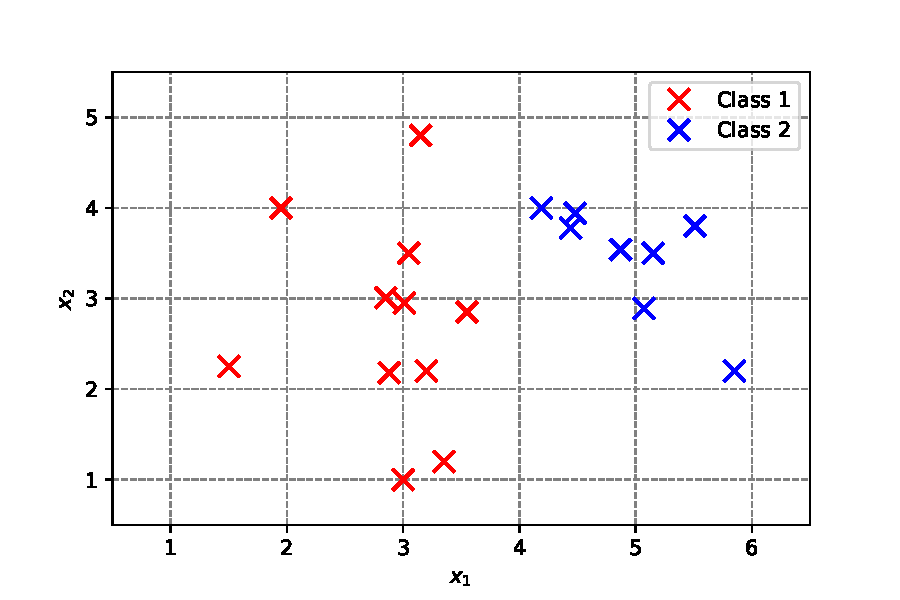
\includegraphics[scale=0.45]{07_logistic_regression/02_img/logreg_example_linear}
		\end{figure}
	}{0.49}{
		\begin{figure}
			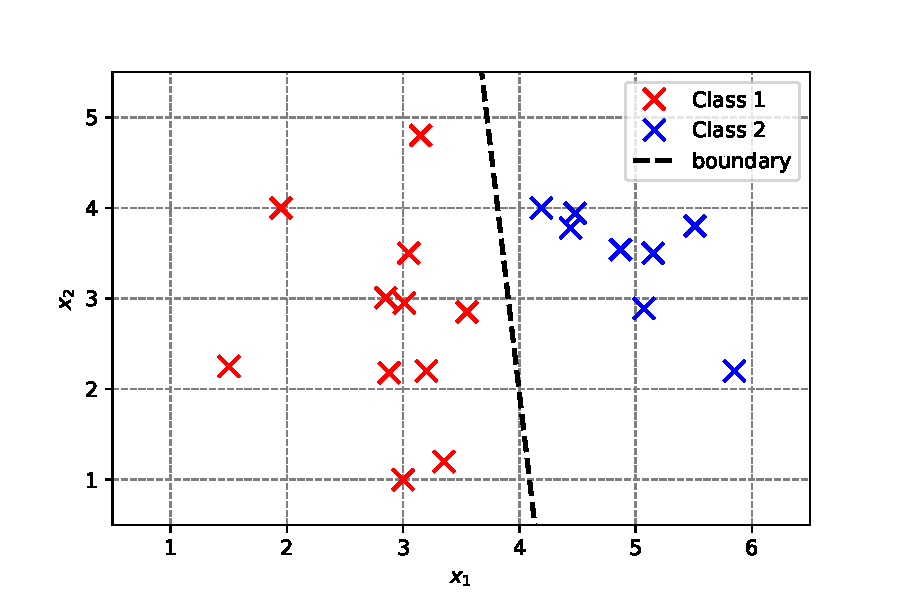
\includegraphics[scale=0.45]{07_logistic_regression/02_img/logreg_example_linear_boundary}
		\end{figure}
	}
	
	\begin{center}
		\highlight{Where is the sigmoid function?}
	\end{center}
\end{frame}


% Example: Logistic Function
\begin{frame}{Example: Logistic Function}{}
	\vspace*{-7mm}
	\begin{figure}
		\centering
		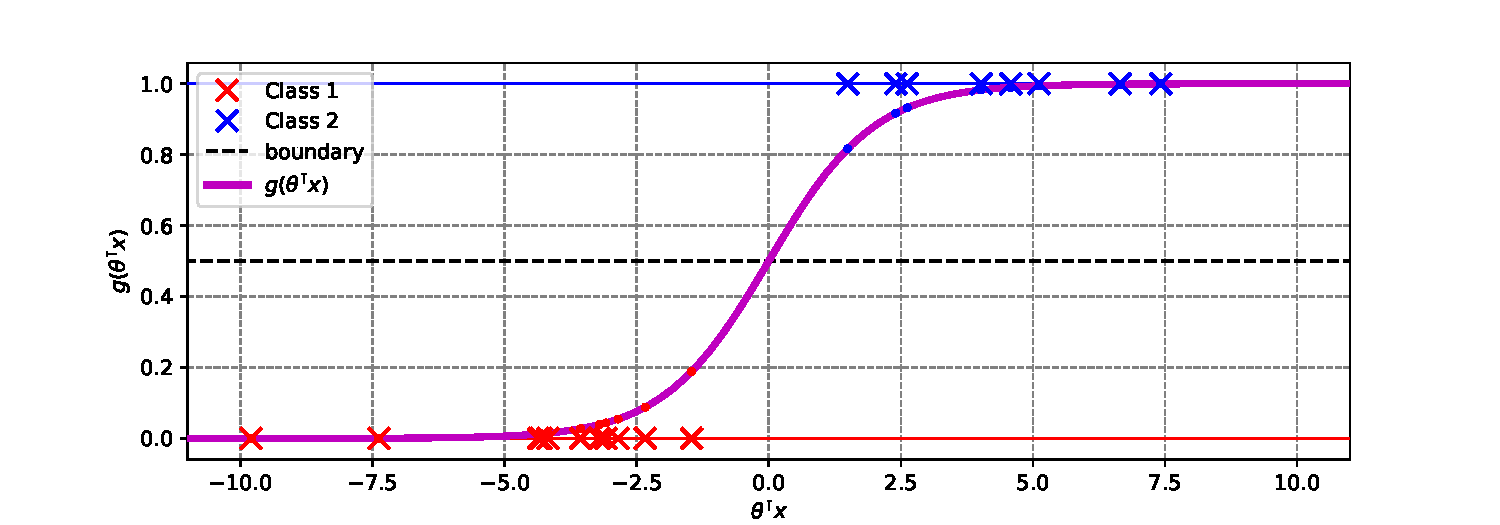
\includegraphics[scale=0.6]{07_logistic_regression/02_img/logreg_example_linear_logistic_function}
	\end{figure}
\end{frame}


% Section: Non-linear Data
%______________________________________________________________________
\section{Non-linear Data}
\makedivider{Non-linear Data}

% Subsection: Feature Mapping
% --------------------------------------------------------------------------------------------------------
\subsection{Feature Mapping}

% Non-Linear Decision Boundaries
\begin{frame}{Non-Linear Decision Boundaries}{}
	\begin{itemize}
		\item \highlight{Feature mapping} can be used to obtain non-linear decision boundaries
		\item \textbf{Example:}
		\begin{itemize}
			\item Imagine a circular data set
			\item Using the features...
			\begin{equation*}
				h_{\bm{\theta}}(\bm{x}) = g(\theta_0 + \theta_1 x_1 + \theta_2 x_2 +
				\textcolor{myblue1}{\theta_3 x_1^2} + \textcolor{myblue1}{\theta_4 x_2^2})
			\end{equation*}
			\item ...the algorithm could e.\,g. choose: $\bm{\theta} =
				\begin{bmatrix} -1, 0, 0, 1, 1 \end{bmatrix}^{\intercal}$
			\item So we would get: $x_1^2 + x_2^2 = 1 \Rightarrow$ \textbf{equation of a unit circle}
		\end{itemize}
	\end{itemize}
\end{frame}


% Example: Non-Linear Decision Boundary
\begin{frame}{Example: Non-Linear Decision Boundary}{}
	\vspace*{-2mm}
	\begin{figure}
		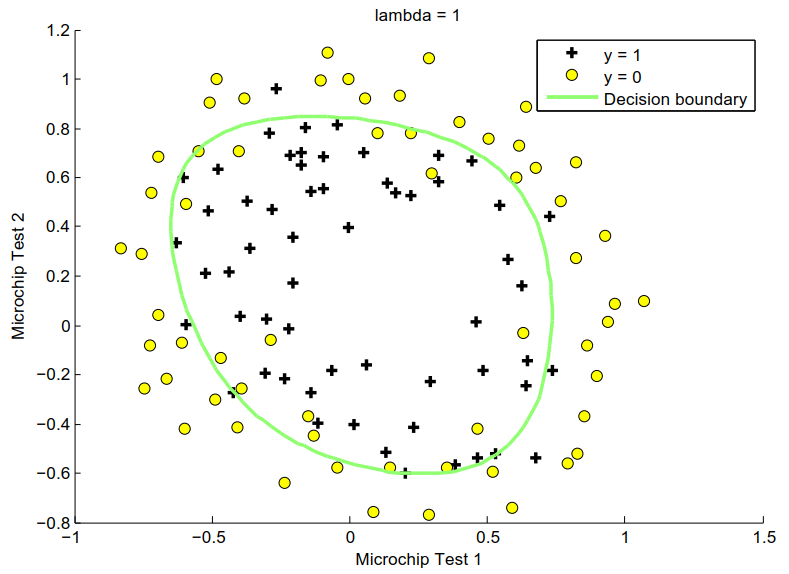
\includegraphics[scale=0.325]{07_logistic_regression/02_img/logreg_example_non_linear_boundary}
	\end{figure}
\end{frame}


% Subsection: Regularization
% --------------------------------------------------------------------------------------------------------
\subsection{Regularization}

% Logistic Regression Cost Function (Ctd.)
\begin{frame}{Logistic Regression Cost Function (Ctd.)}{}
	\begin{itemize}
		\item We should apply regularization for non-linear decision boundaries:
		\footnotesize
		\begin{equation}
			\frac{1}{n} \sum_{i=1}^n \left[
				-y^{(i)} \log(h_{\bm{\theta}}(\bm{x}^{(i)})) - (1 - y^{(i)}) \log(1 - h_{\bm{\theta}}(\bm{x}^{(i)}))
			\right] + \textcolor{myblue1}{\frac{\lambda}{2m} \sum_{j=1}^m \theta_j^2}
		\end{equation}
		\normalsize
		\item The last term prevents the parameters $\theta_j$ from becoming too large
		\item $\lambda \ge 0$ controls the degree of regularization
		\item This leads to smoother decision boundaries
	\end{itemize}
\end{frame}


% Section: Multi-Class Classification
%______________________________________________________________________
\section{Multi-Class Classification}
\makedivider{Multi-Class Classification}

% Subsection: Multiple Classes
% --------------------------------------------------------------------------------------------------------
\subsection{Multiple Classes}

% Multi-Class Classification
\begin{frame}{Multi-Class Classification}{}
	\begin{itemize}
		\item Logistic regression can handle two classes only, namely \textbf{0} and \textbf{1}
		\item \textbf{What if there are more than two classes?}
		\item Two common techniques:
		\begin{itemize}
			\item \highlight{One-vs-Rest (OVR)} 	$\Rightarrow$ One-against-All
			\item \highlight{One-vs-One (OVO)} 	$\Rightarrow$ Pairwise classification
		\end{itemize}
		\item Several classifiers are trained
		\item During prediction the classifiers \textbf{vote for the correct class}
		\item Such techniques can be used for all binary classifiers
	\end{itemize}
\end{frame}


% Subsection: One-vs-Rest (OVR)
% --------------------------------------------------------------------------------------------------------
\subsection{One-vs-Rest (OVR)}

% Multi-Class Classification: One-vs-Rest (OVR)
\begin{frame}{Multi-Class Classification: One-vs-Rest (OVR)}{}
	\divideTwo{0.49}{
		\begin{itemize}
			\item \textbf{Train one classifier per class} (expert for that class)
			\item We get $\vert \mathcal{C} \vert$ classifiers
			\item The $k$-th classifier learns to distinguish the $k$-th class from all the others
			\item Set the labels of examples from class $k$ to \textbf{1}, all the others to \textbf{0}
		\end{itemize}
	}{0.49}{
		\vspace*{2mm}
		\begin{figure}
	\centering
	\begin{tikzpicture}[
		scale=0.8
	]

		\begin{axis}[
			xlabel={$x_1$},
			ylabel={$x_2$}
		]
		
			\addplot[
				only marks,mark=*,mark size=2.0,fill=red,discard if not={c}{0}
			] table{07_logistic_regression/05_data/data_multi_class.txt};

			\addplot[
				only marks,mark=*,mark size=2.0,fill=blue,discard if not={c}{1}
			] table{07_logistic_regression/05_data/data_multi_class.txt};

			\addplot[
				only marks,mark=*,mark size=2.0,fill=green,discard if not={c}{2}
			] table{07_logistic_regression/05_data/data_multi_class.txt};

			\draw[thick,dashed,red] (axis cs: -15,-24) -- (axis cs: -3,0) -- (axis cs: -15,30);
			\node[red] at (axis cs: -10,-6) {\textbf{1}};
			\node at (axis cs: 0,0) {\textbf{0}};
			
    		\end{axis}
		
	\end{tikzpicture}
\end{figure}
	}
\end{frame}


% Subsection: One-vs-One (OVO)
% --------------------------------------------------------------------------------------------------------
\subsection{One-vs-One (OVO)}

% Multi-Class Classification: One-vs-One (OVO)
\begin{frame}{Multi-Class Classification: One-vs-One (OVO)}{}
	\divideTwo{0.49}{
		\vspace*{2mm}
		\begin{figure}
	\centering
	\begin{tikzpicture}[
		scale=0.8
	]

		\begin{axis}[
			xlabel={$x_1$},
			ylabel={$x_2$}
		]
		
			\addplot[
				only marks,mark=*,mark size=2.0,fill=red,discard if not={c}{0}
			] table{11_svm/05_data/data_multi_class.txt};

			\addplot[
				only marks,mark=*,mark size=2.0,fill=blue,discard if not={c}{1}
			] table{11_svm/05_data/data_multi_class.txt};

			\addplot[
				only marks,mark=*,mark size=2.0,fill=white,draw=gray,discard if not={c}{2}
			] table{11_svm/05_data/data_multi_class.txt};

			\draw[thick,dashed,red] (axis cs: -10,-10) -- (axis cs: 5,7.5);
			\node[red] at (axis cs: -10,-6) {\textbf{+1}};
			\node[blue] at (axis cs: -5,-7.5) {\textbf{-1}};
			\node[gray] at (axis cs: -2.5,7.5) {ignored};
			
    		\end{axis}
		
	\end{tikzpicture}
\end{figure}
	}{0.49}{
		\begin{itemize}
			\item \textbf{Train one classifier for each pair of classes}
			\item We get $\binom{\vert \mathcal{C} \vert}{2}$ classifiers
			\item Ignore all other examples that do not belong to either of the two classes
			\item \textbf{Voting}: Count how often each class wins; the class with the highest score is predicted
		\end{itemize}
	}
\end{frame}


% Section: Wrap-Up
%______________________________________________________________________
\section{Wrap-Up}
\makedivider{Wrap-Up}

% Subsection: Summary
% --------------------------------------------------------------------------------------------------------
\subsection{Summary}

% Summary
\begin{frame}{Summary}{}
	\begin{itemize}
		\item \Highlight{Logistic regression is used for classification (!!!)}
		\item It is used for \textbf{binary classification problems} (generalizations exist)
		\item \textbf{Output:} Probability of instance belonging to positive class
		\item Apply a \textbf{threshold} to get the classification
		\item The algorithm minimizes the \textbf{cross entropy cost function}
		\item There is \textbf{no closed-form solution} (unlike for linear regression)
		\item \textbf{Basis functions} can be used for non-linear data
		\item \textbf{Multi-class classification:} One-vs-Rest, One-vs-One
	\end{itemize}
\end{frame}


% Subsection: Self-Test Questions
% --------------------------------------------------------------------------------------------------------
\subsection{Self-Test Questions}

% Self-Test Questions
\begin{frame}{Self-Test Questions}{}\important
	\begin{enumerate}
		\item Why should you not use linear regression for classification?
		\item State the formula for the logistic function.
		\item Why do we use cross entropy instead of the squared error?
		\item Does logistic regression find the best-separating hyper-plane?
		\item What techniques do you know for multi-class classification problems?
	\end{enumerate}
\end{frame}


% Subsection: Lecture Outlook
% --------------------------------------------------------------------------------------------------------
\subsection{Lecture Outlook}

\begin{frame}{What's next...?}{}
	\makeoverview{6}
\end{frame}


% Subsection: Recommended Literature and further Reading
% --------------------------------------------------------------------------------------------------------
\subsection{Recommended Literature and further Reading}

% Literature
%______________________________________________________________________
\begin{frame}[allowframebreaks]{Recommended Literature and further Reading}{}
	\footnotesize
	\begin{thebibliography}{2}
		\literature{book}{Bishop.2006}{[2] Pattern Recognition and Machine Learning}
			{Christopher Bishop. Springer. 2006.}{$\rightarrow$ \href{
				http://users.isr.ist.utl.pt/~wurmd/Livros/school/Bishop\%20-\%20Pattern\%20Recognition\%20And\%20Machine\%20Learning\%20-\%20Springer\%20\%202006.pdf
			}{\linkstyle{Link}}, cf. chapter 4.3.2}

		\literature{book}{Murphy.2012}{[2] Machine Learning: A Probabilistic Perspective}
			{Kevin Murphy. MIT Press. 2012.}{$\rightarrow$ \href{
				https://doc.lagout.org/science/Artificial\%20Intelligence/Machine\%20learning/Machine\%20Learning_\%20A\%20Probabilistic\%20Perspective\%20\%5BMurphy\%202012-08-24\%5D.pdf
			}{\linkstyle{Link}}, cf. chapter 8}
	\end{thebibliography}
\end{frame}


% Subsection: Meme of the Day
% --------------------------------------------------------------------------------------------------------
\subsection{Meme of the Day}

% Meme of the Day
\begin{frame}{Meme of the Day}{}
	\begin{figure}
		
\includegraphics[scale=0.45]{07_logistic_regression/02_img/meme_of_the_day}
	\end{figure}
\end{frame}


% Thank you
%______________________________________________________________________
\makethanks

\end{document}